
\chapter{CONTROLLERS}
\label{chap:Controllers}

The control requirements for NASA MMS TableSat 1A can be simplified into three main goals.

First is to maintain a steady spin rate of 3 rpm ($\pi/10$ rad/sec).  Given the relative success of the body rate estimation in Section \ref{chap:Estimators}, this goal should be attainable without the need of advanced control efforts.

Second is to correct for any nutation detected by the estimator.  This requirement can take the form of both driving body rates $\omega_y$ and $\omega_z$ to zero, and ensuring the estimated quaternion's Euler axis is kept in line with the global reference frame's $z$-axis.

Third is to prevent and/or remove oscillations in the Axial Double Probe (ADP) and Spin-plane Double Probe (SDP) booms.  Out of the three, this performance goal has the largest set of dependencies for success.  This level of control is reliant on effective actuators along with reliable state estimates based on an accurate system model which include boom dynamics.

The first two goals is addressed in this chapter as their scope is limited to controller design.  Section \ref{sec:ActuatorConfiguration} covers the configuration of the actuators on TableSat and how their configuration is incorporated into the controller code.  The remaining sections of this chapter focus on the rate and nutation control methods, and use the assumption that the estimators are providing perfect state measurements.  This temporarily limits the scope of the testing to ensure that the control techniques are being implemented properly in the software especially since with the development of some non-standard techniques.  The boom oscillations control goal is addressed in Chapter \ref{chap:ObserverBasedControls} when multiple modules are be linked together to get a wider view of the interactions between sections of observer-based controller acting on noisy state measurements.

\section{Actuator Configuration}
\label{sec:ActuatorConfiguration}

The actuators in use on NASA MMS TableSat 1A consists of four single directional computer fans.  Two oriented for rate control and two for nutation control.  The body rate control fans are mounted on opposite sides of the bus with their thrusts applying opposing moments.  The two nutation fans are mounted flush with the bus at a 90 degree offset and have their thrust directed down.  The fans are assumed to be mounted such that the moments are applied about orthogonal axes.  This simplifies the actuator module's voltage calculations for each fan which can be improved if testing shows the effects are significant enough to compensate for.  Four analog ports to the Athena PC are available for actuator usage after mounting the sensors.  Two dedicated to the rotational fans to provide full rotational control, and the remaining two provide partial nutation control.
\begin{figure}[H]
  \centerline{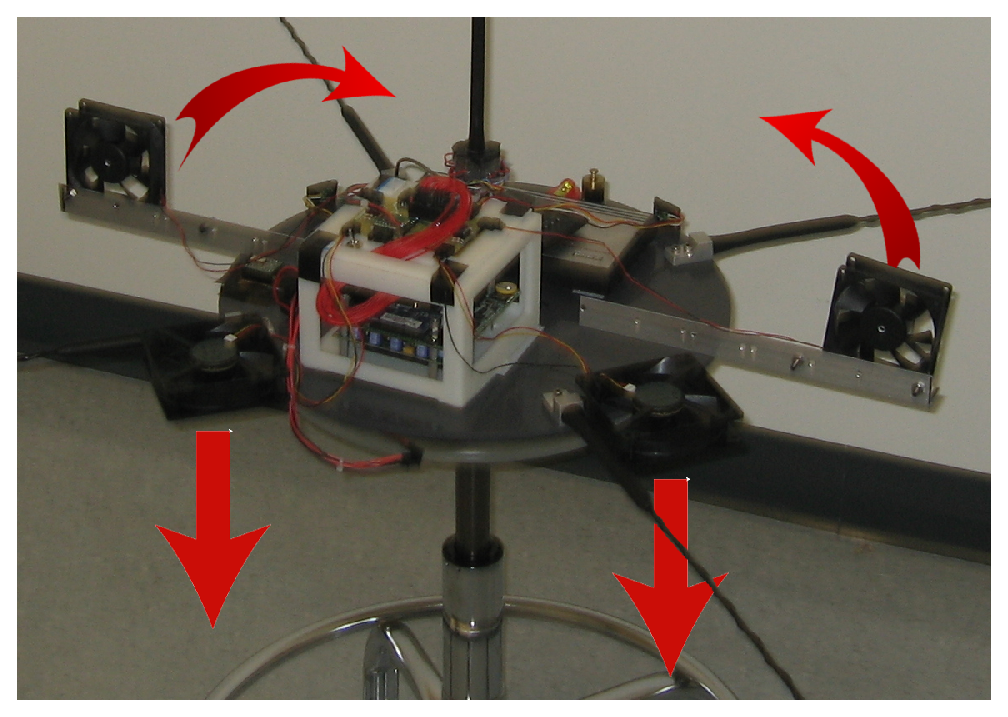
\psfig{file=figures/tsat_thrusters.eps,height=3in}}
  \caption{NASA MMS TableSat 1A thrusters}
  \label{fig:TSatThrusters}
\end{figure}
Passing the desired moments from the controller directly to the estimator without taking the fan geometry into consideration would create a disconnect between the estimated and actual system states.  The software's actuator module is designed to accept a list of fans with their center, direction of thrust related to the body reference frame, and maximum force to determine the moments couples that are actually possible.
\begin{figure}[H]
  \centerline{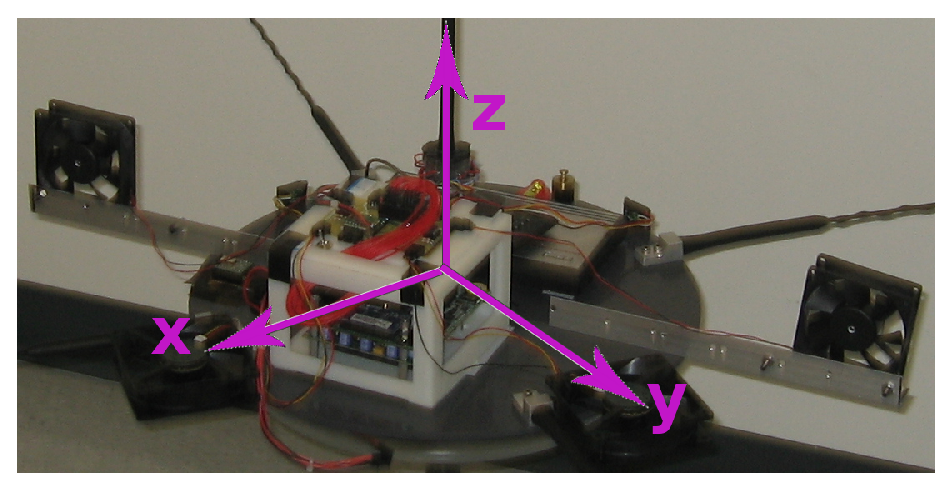
\psfig{file=figures/tsat_body_axes.eps,height=3in}}
  \caption{NASA MMS TableSat 1A Body Axes}
  \label{fig:TableSatBodyAxes}
\end{figure}
Table \ref{tbl:ActuatorConfiguration} shows the fan configuration for the NASA MMS TableSat 1A as arranged in Figure \ref{fig:TSatThrusters}.
\begin{table}[H]
  \centering
  \begin{tabular}{c|c|c|c|c}
    Fan & Center $\bs{f_c}$ (m) & Direction $\bs{n}$ & $F$ (N) & Max Moment $\frac{F \bs{n} \times \bs{f_c}}{|\bs{n}|}$ (Nm) \\ \hline
    1 & $(0.2474, -0.2474, 0)$ & $(-1, -1, 0)$ & 0.08 & $(0, 0, 0.039598)$ \\
    2 & $(-0.2474, 0.2474, 0)$ & $(-1, -1, 0)$ & 0.08 & $(0, 0, -0.039598)$ \\
    3 & $(0.25, 0, 0)$ & $(0, 0, -1)$ & 0.08 & $(0.02, 0, 0)$ \\
    4 & $(0, 0.25, 0)$ & $(0, 0, -1)$ & 0.08 & $(0, -0.02, 0)$ \\
  \end{tabular}
  \caption{Actuator configuration}
  \label{tbl:ActuatorConfiguration}
\end{table}
The code snippet below demonstrates the actuator module's functionality as it has been implemented in the TSatPy software.  Lines 4-13 define the geometry of the actuators displayed in Figure \ref{fig:TSatThrusters} with the addition of a hypothetical fifth actuator along with their center, direction of thrust, and maximum thrust force.

\begin{singlespace}
  \begin{minted}[mathescape,linenos,numbersep=10pt,frame=lines,framesep=2mm]{python}
import numpy as np
from TSatPy.Actuator import Actuator

configs = [{'type': 'fan', 'args': {'name': 'CW',
  'center': (0.2474, -0.2474, 0), 'direction': (-1, -1, 0), 'F': 0.08}
},{'type': 'fan', 'args': {'name': 'CCW1',
  'center': (-0.2474, 0.2474, 0), 'direction': (-1, -1, 0), 'F': 0.08}
},{'type': 'fan', 'args': {'name': 'CCW2',
  'center': (-0.2474, -0.2474, 0), 'direction': (1, -1, 0), 'F': 0.08}
},{'type': 'fan', 'args': {'name': 'NY', 'center': (0.25, 0, 0),
  'direction': (0, 0, 1), 'F': 0.08}
},{'type': 'fan', 'args': {'name': 'NX', 'center': (0, 0.25, 0),
  'direction': (0, 0, 1), 'F': 0.08}}]

def set_level(act, power_level):
    print 'Setting power level=%g for: %s' % (power_level, act)

def setup_actuators(configs):
    act = Actuator()
    for config in configs:
        act.add(config['type'], set_level, config['args'])
    return act

act = setup_actuators(configs)
print(act)
M = np.mat([0.03, 0.11, 0.04]).T
print("Request moment: %s" % (M.T))
print("Applied moment: %s" % (act.request_moment(M).T))

# Prints Out
# Actuator
#  <Fan CW moment=(0, -0, -0.0279901)>
#  <Fan CCW1 moment=(0, 0, 0.0279901)>
#  <Fan CCW2 moment=(0, 0, 0.0279901)>
#  <Fan NY moment=(0, -0.02, 0)>
#  <Fan NX moment=(0.02, 0, 0)>
# Request moment: [[ 0.03  0.11  0.04]]
# Setting power level=1 for: <Fan NX moment=(0.02, 0, 0)>
# Setting power level=0.714538 for: <Fan CCW1 moment=(0, 0, 0.0279901)>
# Setting power level=0.714538 for: <Fan CCW2 moment=(0, 0, 0.0279901)>
# Applied moment: [[ 0.02  0.    0.04]]
  \end{minted}
\nocite{minted}
\end{singlespace}

At line 24, the actuator instance is created and each fan's potential contribution to the overall control moment is calculated with
\begin{equation}
  \bs{M} = \frac{F \bs{n} \times \bs{f_c}}{|\bs{n}|}
\end{equation}
The script output shown above describes how a requested moment of $M_x = 0.03Nm, M_y = 0.11Nm, M_z = 0.04Nm$ would be applied to the five fan configuration.  The ``Nx'' fan can only produce a $0.02Nm$ moment, so gets set to full power to supply part of the requested $M_x = 0.03Nm$.  The ``Ny'' fan does not contribute since it's thrust is in the opposite direction from the needed $M_y = 0.11Nm$.  The ``CCW1'' and ``CCW2'' fans can not individually meet the requested $M_z = 0.04Nm$, but are able to collaboratively reach the requested moment by contributing 71\% each.  In the end, the actual moment that would be applied to the s/c is $M_x = 0.02Nm, M_y = 0Nm, M_z = 0.04Nm$.  This actual moment is both converted to voltages to be transmitted to the TableSat and supplied to the feedback loop to update the estimator's state propagation.

\section{Rate Control}
\label{sec:RateControl}

The first of the three controls goals introduced at the start of this chapter, is to attain a body rate of
\begin{equation}
  \bs{\omega}_d = 0 \bs{i} + 0 \bs{j} + 0.314 \bs{k}
\end{equation}
This desired rate is used for the tests in Sections \ref{subsec:PRateControl} through \ref{subsec:SlidingModeController}.  As explained at the start of the chapter, the following iterations of body rate controllers are tested under the assumption of perfect measurements to ensure appropriate functionality before combining with other modules for observer-based controls.
\subsection{P Rate Controller}
\label{subsec:PRateControl}
The initial controller tested is the proportional body rate controller of the form
\begin{equation}
  \bs{M}_{\omega} = \bs{K}_{\omega p} \left( \bs{\hat{\omega}} - \bs{\omega}_d \right)
  \label{eqn:PRateControl}
\end{equation}
Through a series of simulations with randomized initial conditions for body rates a gradient descent based on minimizing control effort is used to tune the proportional gains to
\begin{equation}
  \bs{K}_{\omega p} = \begin{bmatrix} 0.404 & 0 & 0 \\ 0 & 0.463 & 0 \\ 0 & 0 & 0.428 \end{bmatrix}
\end{equation}
Figure \ref{fig:PRateControl} graphs the body rates and applied moments for one of the the optimized gain tests.  The results show an adequate level of control that damps out the $\omega_x$ and $\omega_y$ rotations and maintains the 0.314 rad/sec for $\omega_z$.  Section \ref{subsec:PIDRateControl} expands on the controller to demonstrate the implementation of the integral and derivative components of the PID since the P-controller is susceptible to errors caused by noisy measurements.
\begin{figure}[H]
  \centerline{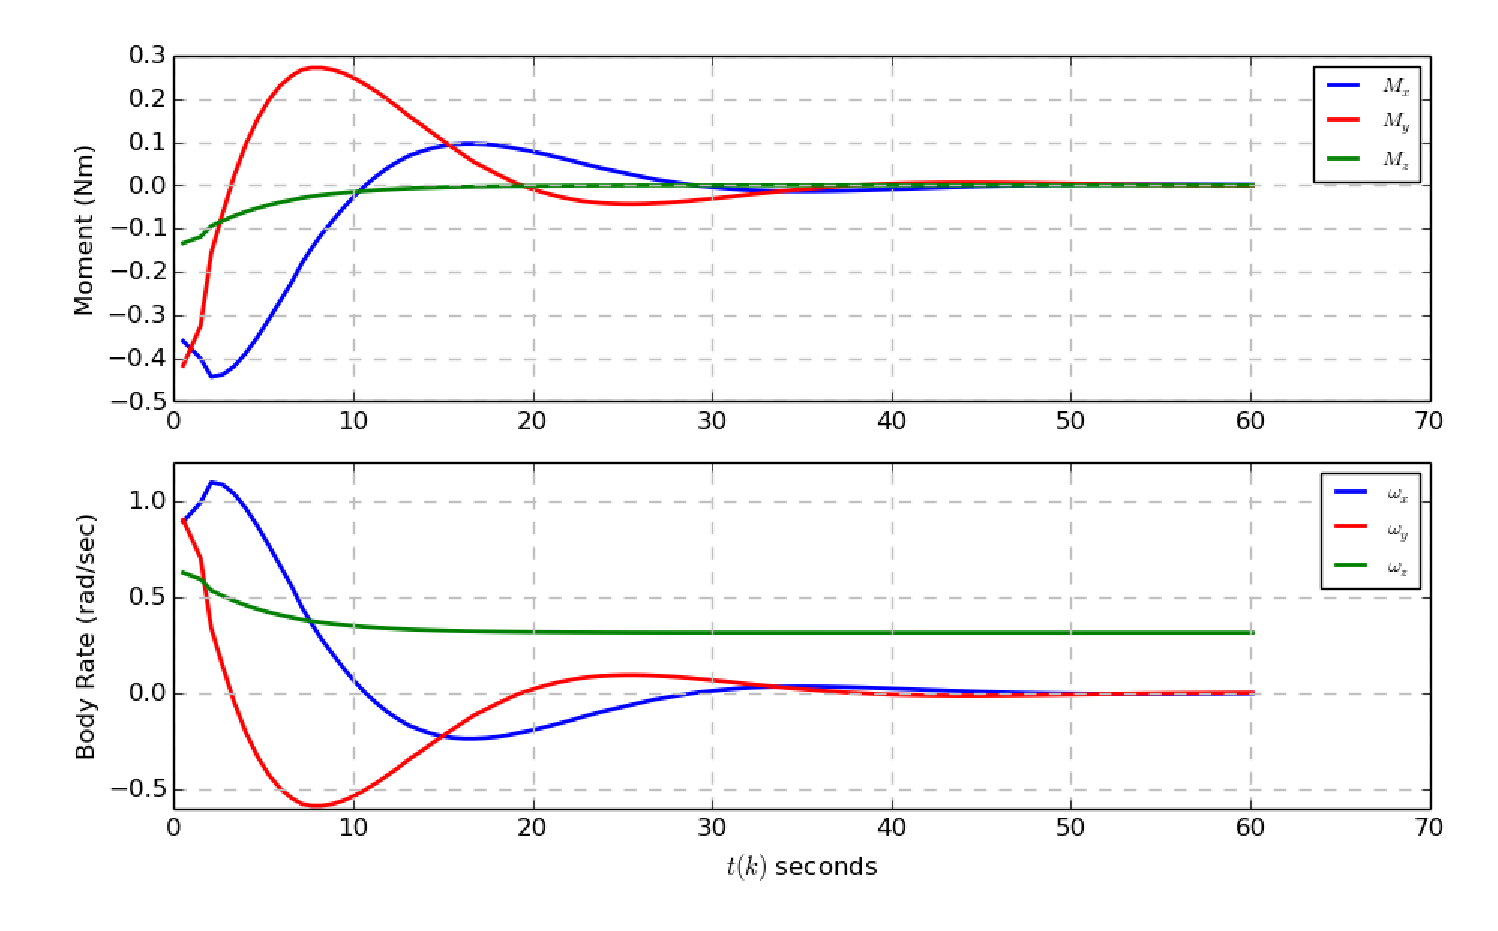
\psfig{file=figures/p_rate_control.eps,width=6in}}
  \caption{P rate control}
  \label{fig:PRateControl}
\end{figure}

\subsection{PID Rate Controller}
\label{subsec:PIDRateControl}

Expanding the proportional controller to include the integral and derivative term as shown in Equation \ref{eqn:PIDRateControl} can improve the performance slightly in the perfect measurement tests, but more importantly provides tools for dealing with noisy measurements when assessing observer-based controllers in Chapter \ref{chap:ObserverBasedControls}.  The integral and derivative terms are implemented with the $\Delta t_k$ adaptive step as with the PID estimator to help account for inconsistencies in update intervals by tracking the step size at each update.
\begin{equation}
  \begin{aligned}
    \bs{M}_{\omega} &= \bs{K}_{\omega p} \bs{\omega}_e + \bs{K}_{\omega i} \cdot (\Delta t_k \bs{I})\cdot \bs{\omega}_e + \bs{K}_{\omega d} \cdot \left(\frac{1}{\Delta t_k} \bs{I}\right) \cdot \bs{\omega}_e
  \end{aligned}
  \label{eqn:PIDRateControl}
\end{equation}
\begin{figure}[H]
  \centerline{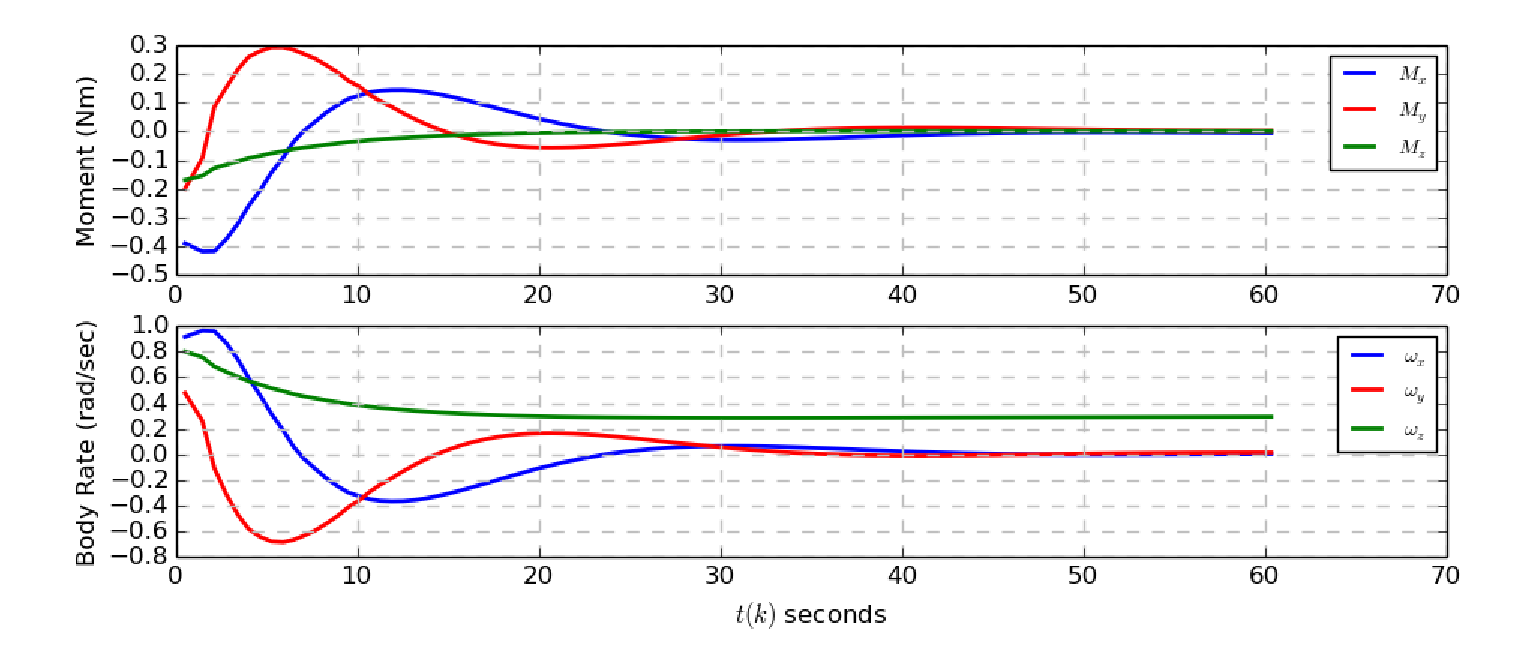
\psfig{file=figures/pid_rate_control.eps,width=6in}}
  \caption{PID rate control}
  \label{fig:PIDRateControl}
\end{figure}
The response curve in Figure \ref{fig:PIDRateControl} is generated from a random initial condition, and with the PID gains (Equation \ref{eqn:PIDRateControlGains}) tuned through gradient descent iterations based on minimizing the total control effort.  In the case of the perfect measurements, the addition correction two control terms generally reduce the overshoot of the response, but do not significantly shorten the time to bring the system to a steady state.
\begin{equation}
  \begin{aligned}
    \bs{K}_{\omega p} &= \begin{bmatrix} 0.424 & 0 & 0 \\ 0 & 0.416 & 0 \\ 0 & 0 & 0.346 \end{bmatrix},
    \bs{K}_{\omega i} = \begin{bmatrix} 0.006 & 0 & 0 \\ 0 & 0.003 & 0 \\ 0 & 0 & 0.005 \end{bmatrix} \\
    \bs{K}_{\omega d} &= \begin{bmatrix} 0.044 & 0 & 0 \\ 0 & 0.072 & 0 \\ 0 & 0 & 0.042 \end{bmatrix}
  \end{aligned}
  \label{eqn:PIDRateControlGains}
\end{equation}
Figure \ref{fig:PIDRateControlMoments} shows how the moments from each of the PID components contributes to the overall moments applied.  The addition of the derivative term gives the system a slightly quicker response that just the P-controller, and in this perfect measurement scenario the the overall performance of the system would benefit from the integral term being removed altogether since it doesn't contribute much to the initial response and even causes a larger steady state error than the P-controller.
\begin{figure}[H]
  \centerline{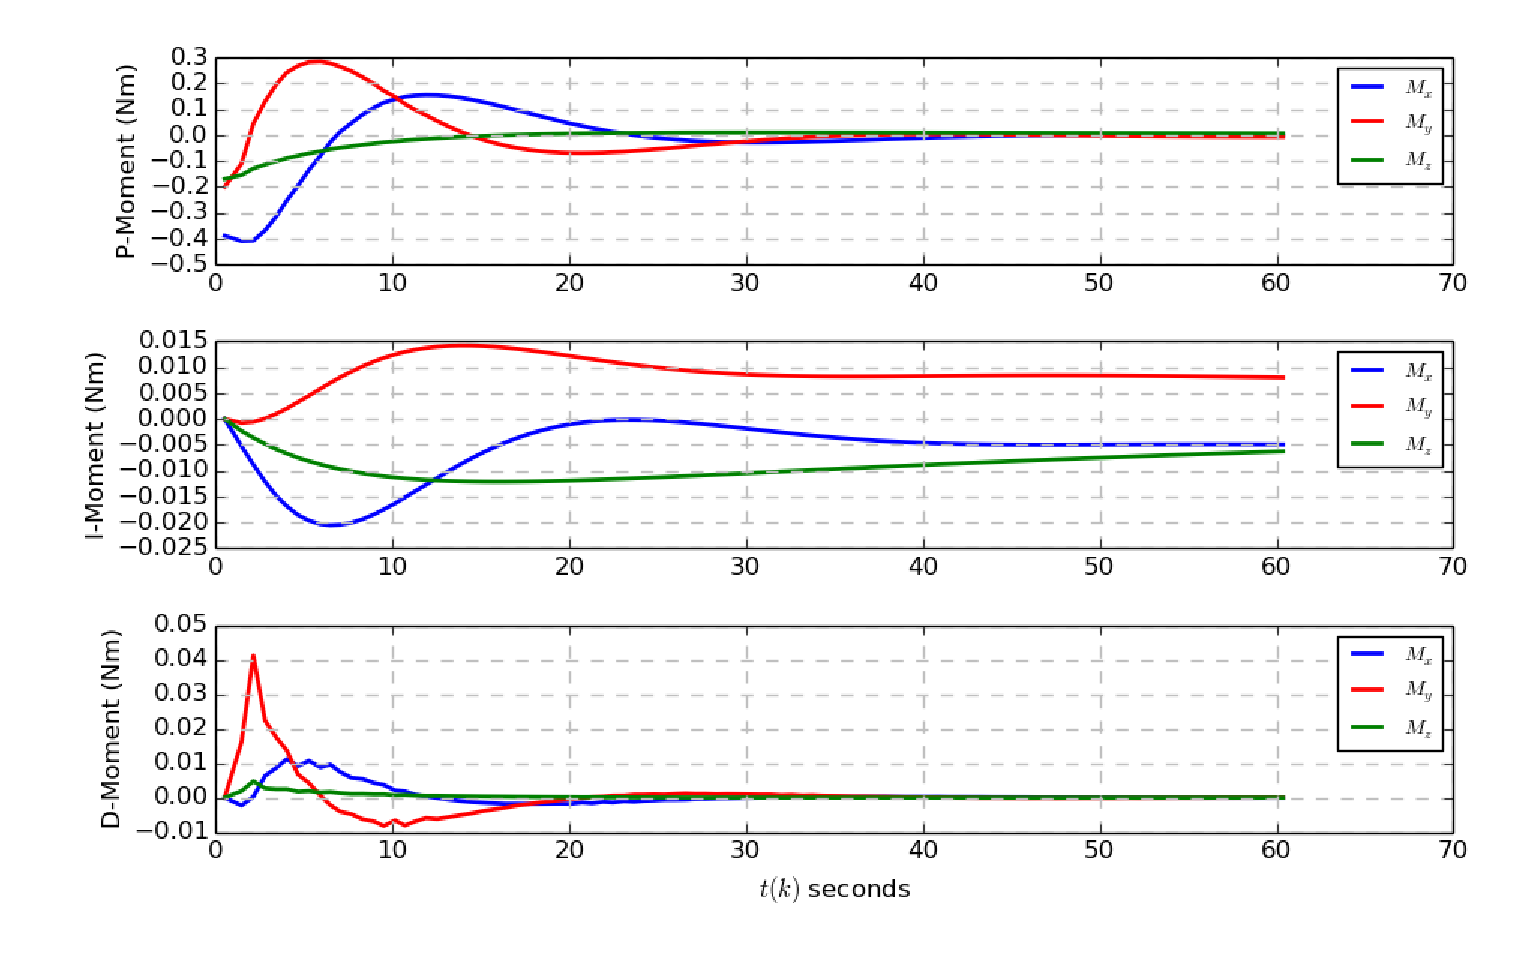
\psfig{file=figures/pid_rate_control_moments.eps,width=6in}}
  \caption{PID rate control moments}
  \label{fig:PIDRateControlMoments}
\end{figure}

\subsection{Sliding Mode Controller}
\label{subsec:SlidingModeController}

The Sliding Mode Controller (SMC) operates similarly to a proportional controller and is governed by the equation
\begin{equation}
  \bs{M}_{\omega} = \bs{L}_{\omega} \bs{\omega}_e + \bs{K}_{\omega}\bs{1}_s \big(\bs{\omega}_e \big)
  \label{eqn:SMController}
\end{equation}
where $\bs{L}_{\omega}$ is the proportional gain and the $\bs{1}_s$ function can take a number of forms such as the signum and arctangent function.  In this thesis, the smc uses the saturation function such that $\bs{1}_s$ is
\begin{equation}
  \bs{1}_s \big(\bs{\omega}_e \big) = sat \begin{bmatrix} \omega_{ex} / S_{\omega} &0 &0 \\ 0 & \omega_{ey} / S_{\omega} & 0 \\ 0 & 0 & \omega_{ez} / S_{\omega} \end{bmatrix}
\end{equation}
The response to the test configuration shows significant improvements in performance over the P and PID rate controller as shown if Figure \ref{fig:SMCRateControl}.
\begin{figure}[H]
  \centerline{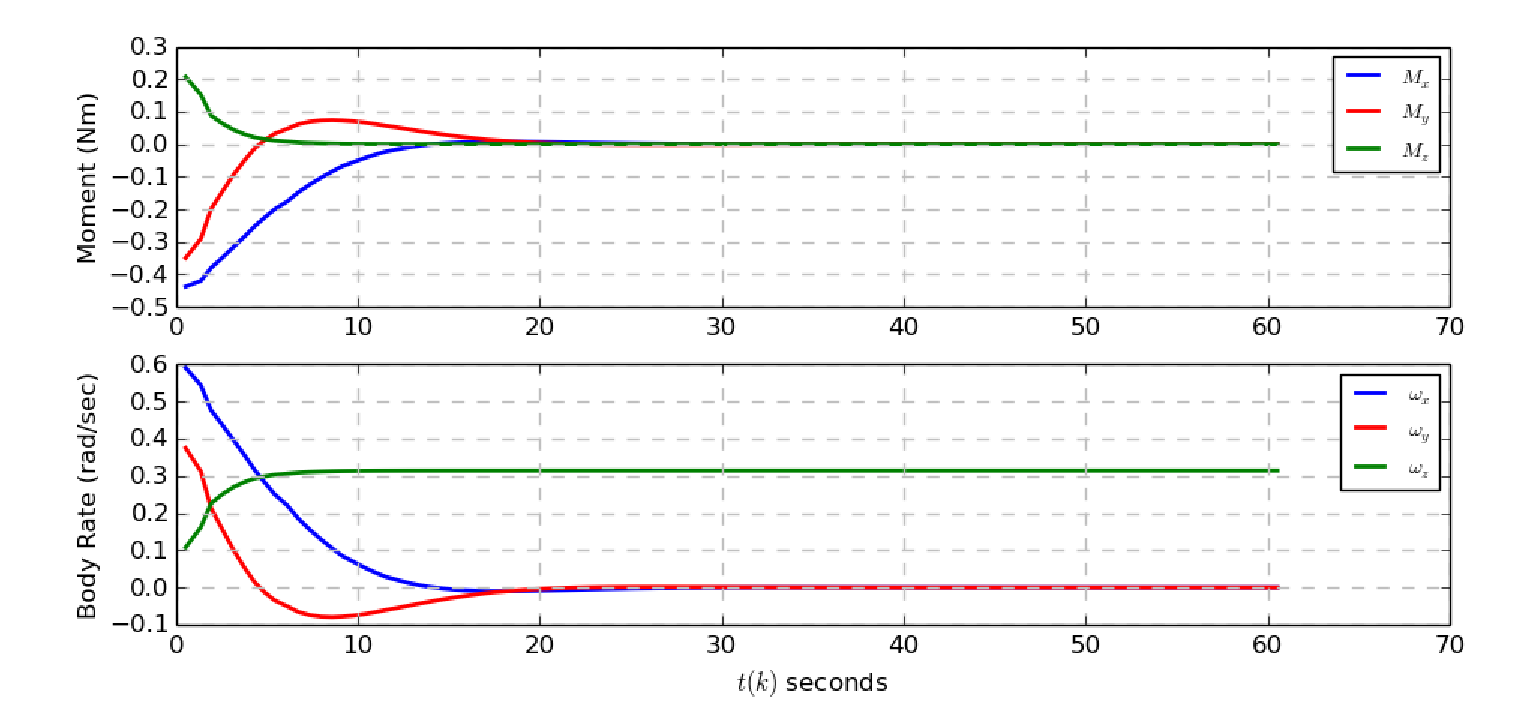
\psfig{file=figures/smc_rate_control.eps,width=6in}}
  \caption{SMC rate control}
  \label{fig:SMCRateControl}
\end{figure}
Breaking the overall moment values into the separate term's contributions (Figure \ref{fig:SMCRateControlMoments}) shows the similar profile between the proportional and saturation term contributions with the exception of the peaks missing from the saturation response.
\begin{figure}[H]
  \centerline{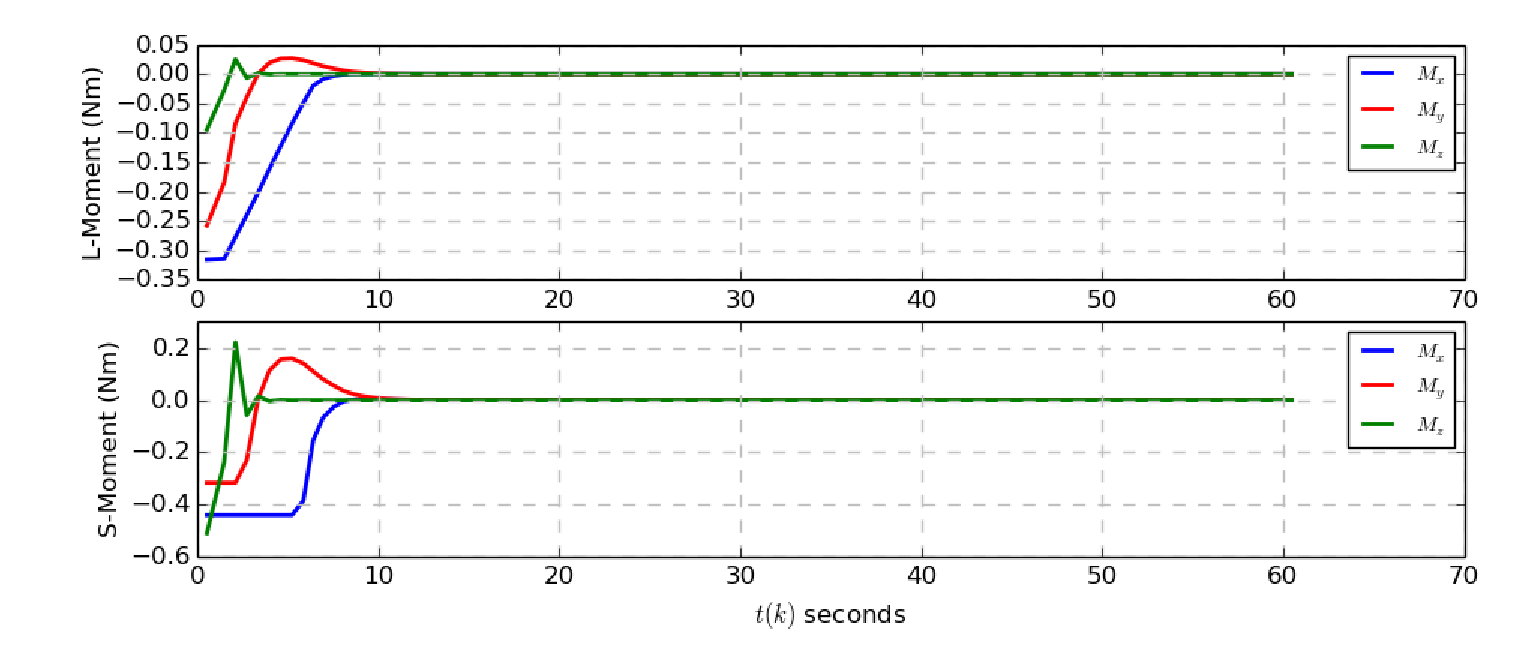
\psfig{file=figures/smc_rate_control_moments.eps,width=6in}}
  \caption{SMC rate control moments}
  \label{fig:SMCRateControlMoments}
\end{figure}
The SMC response in Figures \ref{fig:SMCRateControl} and \ref{fig:SMCRateControlMoments}, is generated with the following gain values tuned through a gradient descent search that minimizes control effort.
\begin{equation}
    \bs{L}_{\omega} = \begin{bmatrix} 0.3983 & 0 & 0 \\ 0 & 0.3828 & 0 \\ 0 & 0 & 0.4160 \end{bmatrix},
    \bs{K}_{\omega} = \begin{bmatrix} 0.4399 & 0 & 0 \\ 0 & 0.5097 & 0 \\ 0 & 0 & 0.3162 \end{bmatrix},
    S_{\omega} = 0.1404
  \label{SMCRateControlGains}
\end{equation}
With the perfect measurements in this test, the saturation term adds a significant performance improvement over the P and PID implementations.  Additionally, with two fewer gain values tuning the SMC is slightly less involved than the PID body rate controller.

\section{Quaternion to Moment Conversion}
\label{sec:QuaternionToMomentConversion}

The remainder of this chapter focuses on the attitude control problem to correct for nutation (Section \ref{sec:AttitudeAndNutationControl}) and the integration of the attitude and rate controller (Section \ref{sec:AttitudeandBodyRateControl}).  The proper conversion from an attitude error measurement to actuator moments is critical to providing a robust control method.

The attitude error measurement is calculated through the quaternion multiplicative method as is established in Section \ref{sec:HighIntegrityStateAdjustments}

\begin{equation}
  \bs{q}_e = \bs{q}_d^* \otimes \bs{\hat{q}}
\end{equation}

Unlike with the estimator where the input and output formats are both quaternions, the quaternion error in the controller $\bs{q}_e$ is composed of four parameters that need to map to three moments values.  The commonly used method for this is to fall back on matrix algebra where

\begin{equation}
  \bs{M}_q = \begin{bmatrix} 3 \times 4 \end{bmatrix} \begin{bmatrix} q_1 & q_2 & q_3 & q_0 \end{bmatrix}^T
  \label{eqn:traditional_attitude_controller}
\end{equation}

There are two main issues with this approach.  First is that the quaternion parameters are sinusoidal in nature, such that the conversion to moment values through the matrix multiplication, the magnitude of the moment do not scale linearly with the magnitude of the attitude error.

The second issue is that the quaternion is comprised of a vector and scalar that provide two separate types of information about the attitude error.  Lumping the two together in a single matrix multiplication ignores the physical representation of their values.  The vector defines the Euler axis which gives the attitude error it's direction.  A vector component with $q_1 = q_3 = 0, q_2 \ne 0$ means that to move the estimated satellite attitude to the desired attitude requires a rotation about just the body-fixed $y$-axis which requires a moment couple in just $M_y$.  This can be represented simply as
\begin{equation}
  \bs{M}_{q} = \bs{v}_e
\end{equation}
This provides a basis for the direction of the moment couple, but since the rotational quaternion is fixed at a unit norm, the magnitude of the vector component varies with the size of the error.  This is compensated for by normalizing the vector.
\begin{equation}
  \bs{M}_{q} = \bs{\hat{e}}_e
  \label{eqn:quat_vector_to_moment}
\end{equation}
With Equation \ref{eqn:quat_vector_to_moment} establishing the direction for the actuator moments, the remaining issue is to determine how to scale the moment couples in relation to the size of the error.  The remaining $q_0$ quantity is a reasonable first choice as
\begin{equation}
  \bs{M}_{q} = kq_{0e} \bs{\hat{e}}_e
\end{equation}
$q_{0e}$, as with the vector, is a sinusoidal measure.  The underlying $\theta$ measure of the quaternion rotation however is a direct measure of the attitude error.  Extracting the $\theta$ measure from $q_{0e}$ and incorporating into the moment calculation yields
\begin{equation}
  \bs{M}_{q} = \left[- k \cos^{-1} (q_{0e}) \right] \bs{\hat{e}}_e
  \label{eqn:QuaternionToMomentConversion}
\end{equation}
This conversion is used throughout all attitude control calculations in the remainder of this chapter and in the observer-based controllers in Chapter \ref{chap:ObserverBasedControls}.










\section{Attitude and Nutation Control}
\label{sec:AttitudeAndNutationControl}

Section \ref{sec:RateControl} covered the design of the rate controller which addresses the first controller goal to maintain a spin rate of $\omega_z = 3$ rpm.  This section ignores the rate control requirement and focuses strictly on the attitude control problem by incorporating the quaternion to moment conversion in Equation \ref{eqn:QuaternionToMomentConversion} into a PID and SMC attitude controller.   Later, section \ref{sec:AttitudeandBodyRateControl} combines the attitude and body rate controls into a single controller.

\subsection{P Attitude Control}
\label{subsec:PAttitudeControl}

Starting with a simplest design of the proportional attitude control, equation \ref{eqn:QuaternionToMomentConversion} can be directly applied as
\begin{equation}
  \bs{M}_{q} = \left[- K_{qp} \cos^{-1} \big(q_{0e} \big) \right] \bs{\hat{e}}_e \\
  \label{eqn:PAttitudeControl}
\end{equation}
This format of the proportional controller provides a significant time savings over the common method in Equation \ref{eqn:traditional_attitude_controller} when optimizing gains since instead of 12 gain values to tune, the controller is limited to a single gain.

To assess the accurate implementation, a the system is initialized to a state of
\begin{equation}
  \bs{x}_0 = \begin{bmatrix} 0 \bs{i} -0.0477 \bs{j} -0.477 \bs{k} +0.8778 \\ 0 \bs{i} -0.01 \bs{j} +0.2 \bs{k} \end{bmatrix}
\end{equation}
which is essentially a 1 radian twist about the $z$-axis with a slight push out of the spin plane with the initial $\omega_y = -0.01$ rad/sec.  The controller is set with a desired state to return the satellite back to the standard attitude where the body-fixed reference frame is aligned with the global reference frame
\begin{equation}
  \bs{q}_d = 0 \bs{i} +0 \bs{j} +0 \bs{k} + 1
\end{equation}
and a chosen proportional gain of
\begin{equation}
  K_{qp} = 0.04
\end{equation}
The results from the test are shown in Figure \ref{fig:PAttitudeControl}.  The simulation ran for 120 seconds.  The top graph displays the calculated moments required to compensate for the attitude error.  As expected, the $M_z$ is shows the P-controller spring like oscillating moments as the satellite twists back and forth.  The center graph displays the $\theta$ measure that quantifies the distance between the current and desired attitude.  With this measure, it's visible that while the majority of the attitude error is linked to the twist about the $z$-axis.  The error gets progressively larger through each rotation as some of the rotational motion gets transferred to the out of plane motion.
\begin{figure}[H]
  \centerline{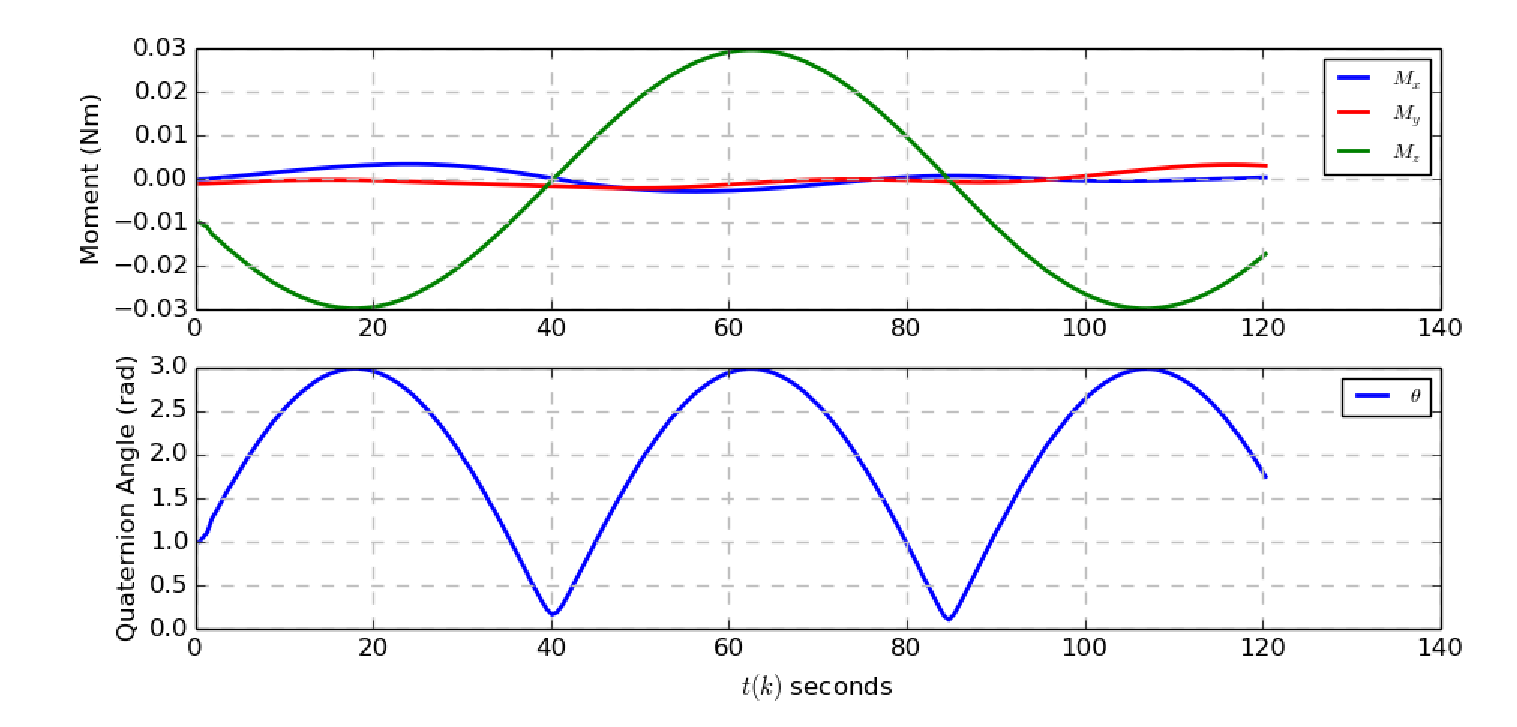
\psfig{file=figures/p_attitude_control.eps,width=6in}}
  \caption{P Attitude Control}
  \label{fig:PAttitudeControl}
\end{figure}








\subsection{Quaternion Decomposition for Nutation Control}
\label{subsec:QuaternionDecompositionForNutationControl}



Prior to combining the attitude control from Section \ref{subsec:PAttitudeControl} with the body rate control from Section \ref{sec:RateControl}, the controller needs to incorporate the quaternion decomposition method in Equation \ref{eqn:quaternion_decomposition_derivation}.  The advantage to incorporating this into a controller is being able to take the quaternion portion of the state error, decompose it into its associated rotation and nutation quaternions, and replace the quaternion error with the nutation quaternion error.  This limits the attitude controller to just worry about correcting for nutation regardless of the rotational position or angular velocity.

The proportional attitude control from Equation \ref{eqn:PAttitudeControl} becomes
\begin{equation}
  \bs{M}_{q} = \left[- K_{qp} \cos^{-1} \big(q_{0en} \big) \right] \bs{\hat{e}}_{en} \\
\end{equation}
where $q_{0en}$ is the scalar component of the error quaternion's nutation component, and $\bs{\hat{e}}_{en}$ is the normalized Euler axis for the nutation component.

The following code snippet shows how the incorporation of this method in the TSatPy software where the state error $x_e$ has its attitude measure adjusted to represent only the nutation error.

\begin{singlespace}
  \begin{minted}[mathescape,linenos,numbersep=10pt,frame=lines,framesep=2mm]{python}
from TSatPy.State import State, Quaternion, BodyRate

print("State Error")
x_e = State(
    Quaternion([0,0.1,1],radians=1),
    BodyRate([0,-0.01,0.2]))
print("x_e: %s" % (x_e))

print("Decomposed Quaternion")
q_r, q_n = x_e.q.decompose()
print("q_r: %s" % q_r)
print("q_n: %s" % q_n)

print("Nutation Only State Error")
x_e.q = q_n
print("x_e: %s" % (x_e))

# Prints Out
# State Error
# x_e: <Quaternion [-0 -0.0477046 -0.477046], 0.877583>,
#      <BodyRate [0 -0.01 0.2]>
# Decomposed Quaternion
# q_r: <Quaternion [0 0 -0.47759], 0.878583>
# q_n: <Quaternion [-0.0227833 -0.0419125 -0], -0.998861>
# Nutation Only State Error
# x_e: <Quaternion [-0.0227833 -0.0419125 -0], -0.998861>,
#      <BodyRate [0 -0.01 0.2]>
  \end{minted}
\nocite{minted}
\end{singlespace}

Now that there is a defined method for separating the allowed rotation from the unwanted nutation, Section \ref{subsec:PNutationControl} shows the decomposition in use with the proportional attitude controller.

\subsection{P Nutation Control}
\label{subsec:PNutationControl}

Using the proportional control
\begin{equation}
  \bs{M}_{q} = \left[- K_{qp} \cos^{-1} (q_{0n}) \right] \bs{\hat{e}}_n
  \label{eqn:PNutationControl}
\end{equation}
with the same initial state and desired quaternion as the proportional attitude controller
\begin{equation}
  \bs{x}_0 = \begin{bmatrix} 0 \bs{i} -0.0477 \bs{j} -0.477 \bs{k} +0.8778 \\ 0 \bs{i} -0.01 \bs{j} +0.2 \bs{k} \end{bmatrix}
\end{equation}
\begin{equation}
  \bs{q}_d = 0 \bs{i} +0 \bs{j} +0 \bs{k} + 1
\end{equation}
\begin{figure}[H]
  \centerline{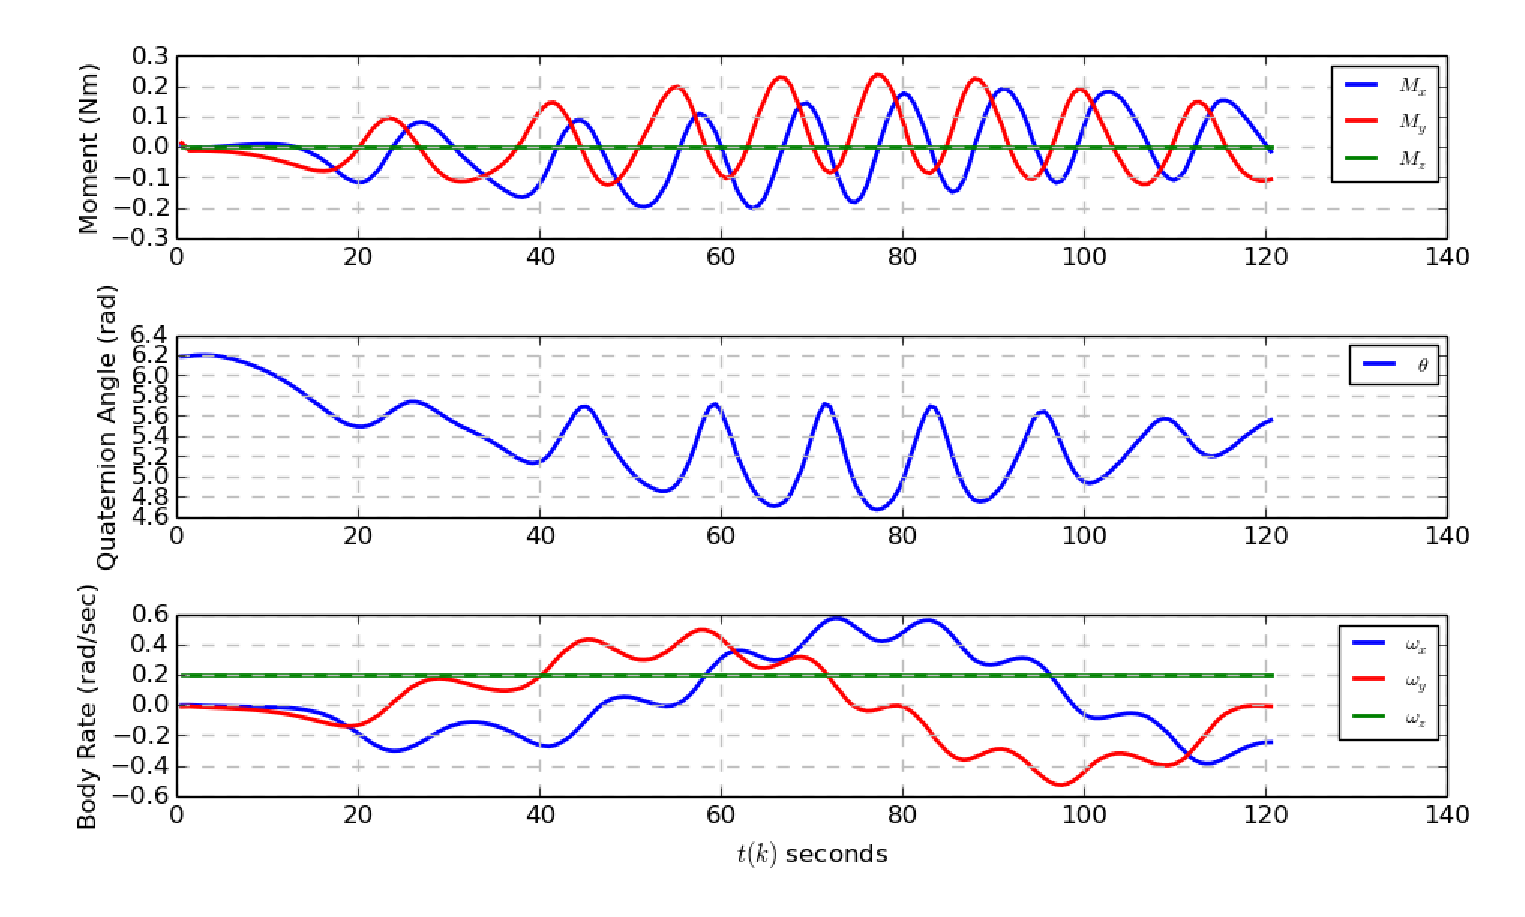
\psfig{file=figures/p_nutation_control.eps,width=6in}}
  \caption{P Nutation Control}
  \label{fig:PNutationControl}
\end{figure}
Figure \ref{fig:PNutationControl} shows the resulting control moments, quaternion angle error, and body rates.  In the first and last graphs, the body rates and moments show the expected behavior where the corrections for initial nutation are causing fluctuations in the $\omega_x$ and $\omega_z$ body rates, but the $\omega_z$ body remains unchanged.  This means that for spin-stabilized systems like NASA's MMS mission satellite, the controller can correct for nutation errors unaffected by the constant spin rate.  The same can be seen in the first graph where moments are applied about the $x$ and $y$ axes, but no attempt is made to control for the initial spin about $z$.
The center plot tracking quaternion angle, shows that while some of the nutation is removed the proportional nutation controller is clearly not enough to remove all nutation.


\section{Attitude and Body Rate Control}
\label{sec:AttitudeandBodyRateControl}

Sections \ref{sec:RateControl} and \ref{sec:AttitudeAndNutationControl} have established methods to address the spin rate and nutation control goals.  In this section the two are used together.  In Section \ref{subsec:FixedAttitudeControl}, the attitude and body rate controllers are combined to take a satellite from an initialized uncontrolled spin and bring it to the standard orientation with fixed-body axes aligned with the global axes.  Section \ref{subsec:SpinStabilizedControl} follows up by releasing the restriction on motion about the $z$ axis and takes the satellite's initial uncontrolled spin to a nutation-free rotation about the $z$-axis.
\begin{equation}
    \bs{M} = \bs{M}_{q} + \bs{M}_{\omega}
\end{equation}
For consistency, all tests in this section are initialized with the following state
\begin{equation}
  \bs{x}_0 = \begin{bmatrix} -0.532 \bs{i} -0.417 \bs{j} -0.275 \bs{k} +0.684 \\ 0.315 \bs{i} +0.207 \bs{j} +0.113 \bs{k} \end{bmatrix}
  \label{eqn:attitude_and_body_rate_control_ic}
\end{equation}

\subsection{Fixed Attitude Control}
\label{subsec:FixedAttitudeControl}
The PID controllers are defined as
\begin{equation}
  \begin{aligned}
    \bs{M} &= \bs{M}_{q} + \bs{M}_{\omega} \\
    \bs{M}_{q} &= \left[- K_{qp} \cos^{-1} (q_{0e}) \right] \bs{\hat{e}}_e + \left[- K_{qi} \cos^{-1} (q_{0ei}) \right] \bs{\hat{e}}_{ei} + \left[- K_{qd} \cos^{-1} (q_{0ed}) \right] \bs{\hat{e}}_{ed} \\
    \bs{M}_{\omega} &= \bs{K}_{\omega p} \bs{\omega}_e + \bs{K}_{\omega i} \cdot (\Delta t_k \bs{I})\cdot \bs{\omega}_e + \bs{K}_{\omega d} \cdot \left(\frac{1}{\Delta t_k} \bs{I}\right) \cdot \bs{\omega}_e
  \end{aligned}
\end{equation}
where $\bs{\hat{e}}_e, \bs{\hat{e}}_{ei}, \bs{\hat{e}}_{ed}$ are the Euler axes for the quaternion error, quaternion error integral, and quaternion error derivative respectively with the integral $\bs{q}_{ei}$ and derivative $\bs{q}_{ed}$ quaternions from Equations \ref{eqn:IEstimator} and \ref{eqn:DEstimator}.

The results from the PID body rate and attitude controller are shown in Figures \ref{fig:PIDAttitudeAndRateControl} and \ref{fig:PIDAttitudeAndRateControlMoments} when tested with the following parameters
\begin{equation}
  \begin{aligned}
    K_{qp} &= 0.6022,K_{qi} = 0.04656,K_{qd} = 0.8554 \\
    K_{\omega p} &= \bs{I} \begin{bmatrix} 0.70326 & 0.7203 & 0.61757 \end{bmatrix}^T \\
    K_{\omega i} &= \bs{I} \begin{bmatrix} 0.04207 & 0.06999 & 0.018591 \end{bmatrix}^T \\
    K_{\omega d} &= \bs{I} \begin{bmatrix} 0.4096 & 0.6032 & 0.6123 \end{bmatrix}^T
  \end{aligned}
\end{equation}
\begin{figure}[H]
  \centerline{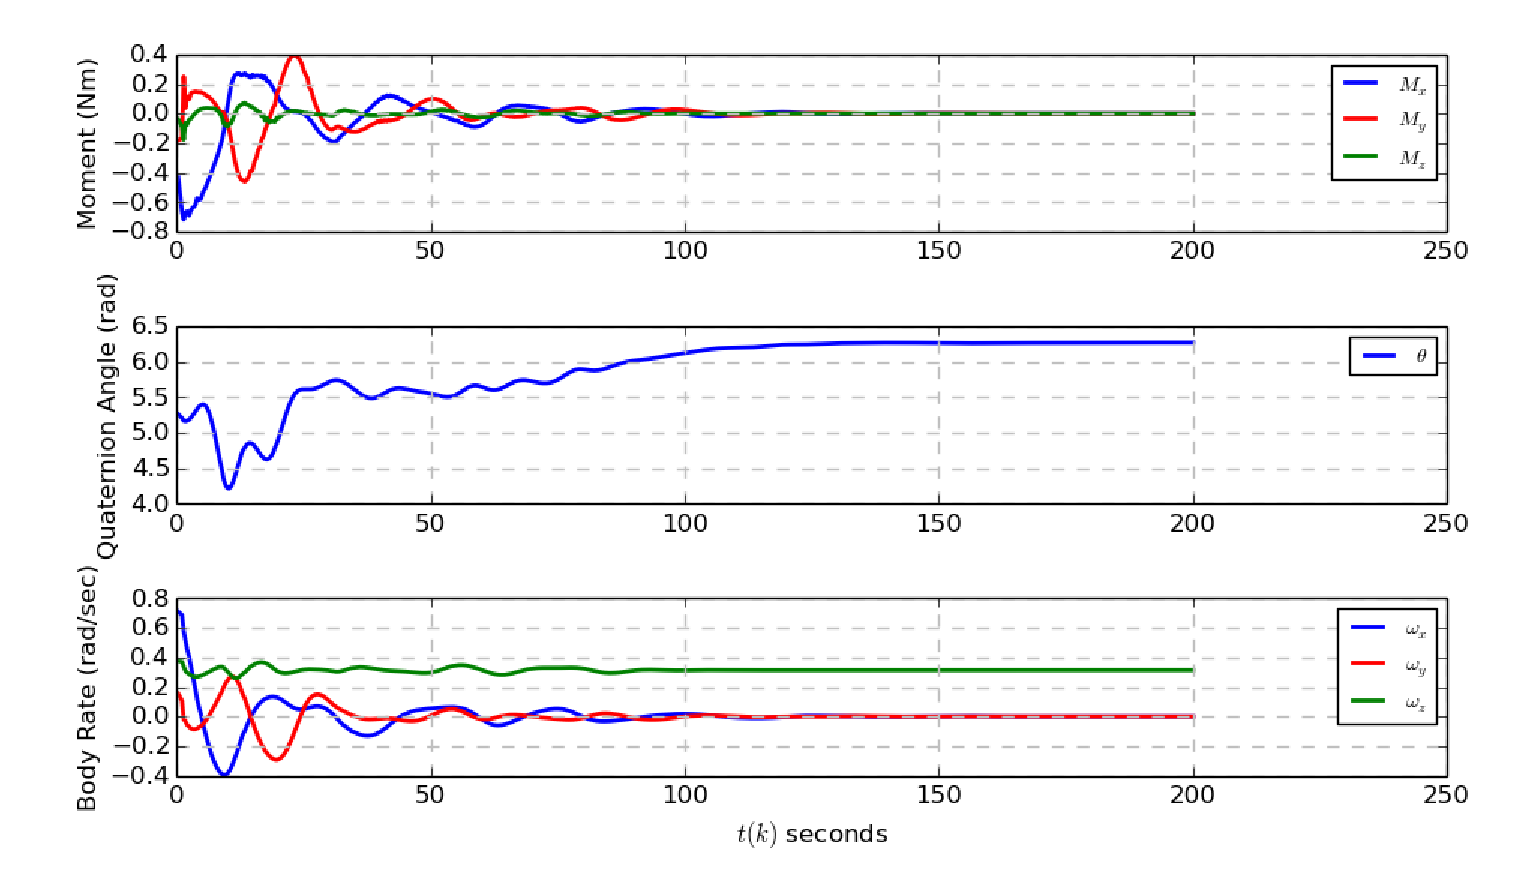
\psfig{file=figures/pid_attitude_and_rate_control.eps,width=6in}}
  \caption{PID Attitude and Rate Control}
  \label{fig:PIDAttitudeAndRateControl}
\end{figure}
Figure \ref{fig:PIDAttitudeAndRateControl} shows a significant improvement to the body rate response over previous body rate only tests.  All error and oscillations in the quaternion angle were also eliminated.  The graphs in \ref{fig:PIDAttitudeAndRateControlMoments} attribute the fast conversion to the desired attitude initially to the proportional and derivative components with the integral component eliminating the final steady state error.
\begin{figure}[H]
  \centerline{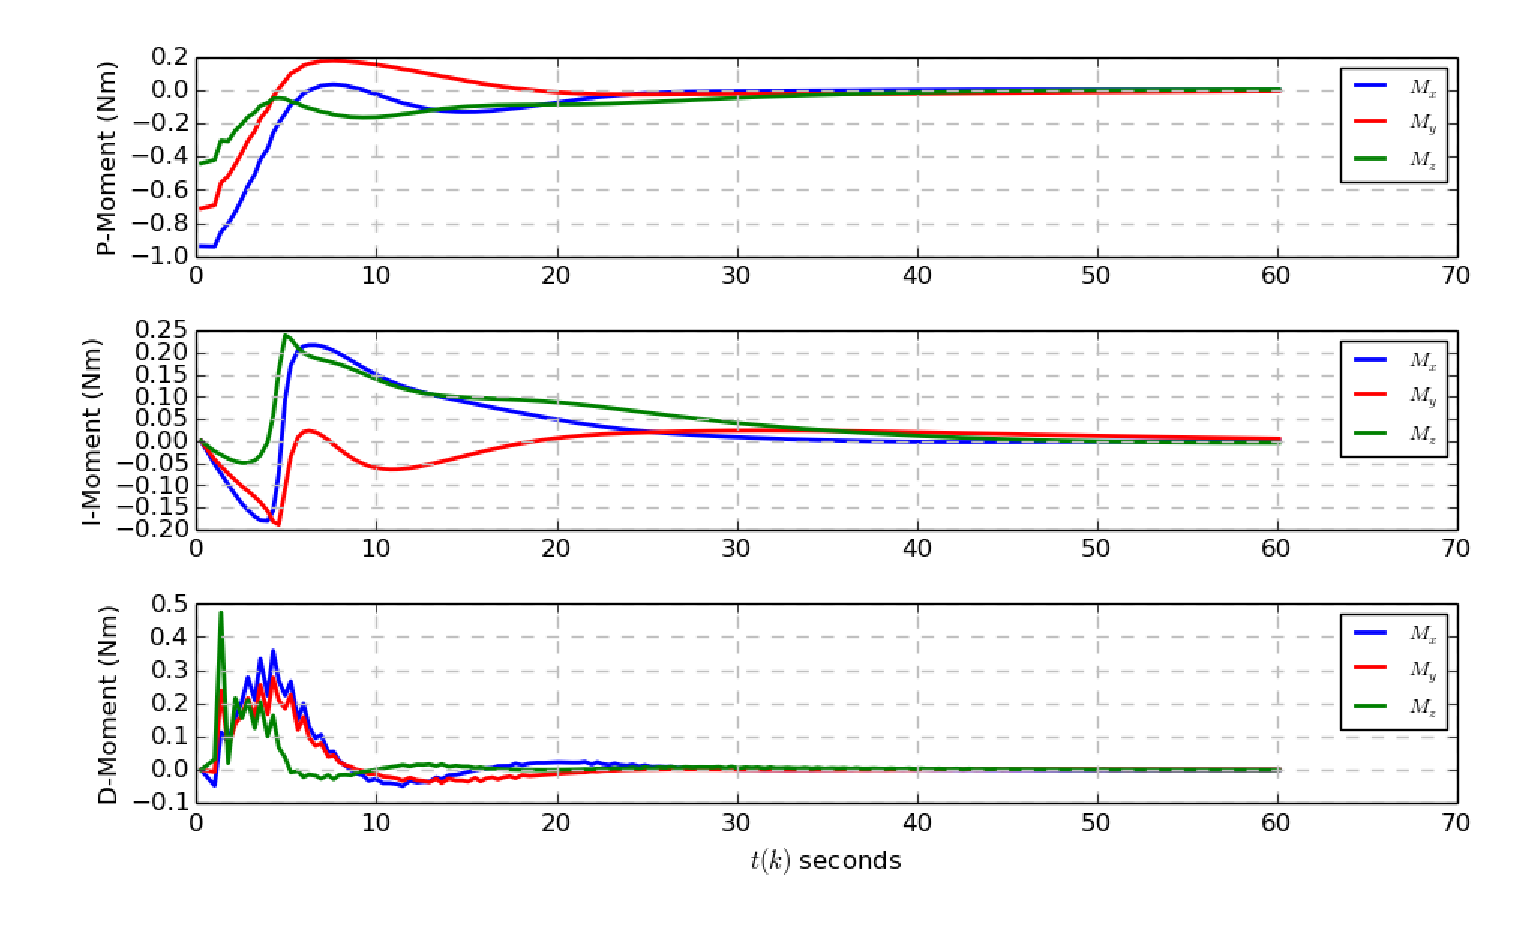
\psfig{file=figures/pid_attitude_and_rate_control_moments.eps,width=6in}}
  \caption{PID Attitude and Rate Control Moments}
  \label{fig:PIDAttitudeAndRateControlMoments}
\end{figure}

The Sliding Mode Controllers are defined as
\begin{equation}
  \begin{aligned}
    \bs{M} &= \bs{M}_{q} + \bs{M}_{\omega} \\
    \bs{M}_{q} &= \left[- L_{q} \cos^{-1} (q_{0e}) \right] \bs{\hat{e}}_e + \left[ K_{q} sat \left( \frac{-2\cos^{-1} (q_{0e})}{S_q} \right) \right] \bs{\hat{e}}_e \\
    \bs{M}_{\omega} &= \bs{L}_{\omega} \bs{\omega}_e + \bs{K}_{\omega}\bs{1}_s \big(\bs{\omega}_e / S_{\omega} \big) \\
    \bs{1}_s \big(\bs{\omega}_e / S_{\omega} \big) &= \begin{bmatrix} sat (\omega_{ex} / S_{\omega}) &0 &0 \\ 0 & sat (\omega_{ey} / S_{\omega}) & 0 \\ 0 & 0 & sat (\omega_{ez} / S_{\omega}) \end{bmatrix}
  \end{aligned}
  \label{eqn:sliding_mode_control}
\end{equation}
Figures \ref{fig:SMCAttitudeAndRateControl} and \ref{fig:SMCAttitudeAndRateControlMoments} show the response for the SMC to the attitude and body rate control test run.  Through a gradient descent search, the SMC parameters are tuned to
\begin{equation}
  \begin{aligned}
    L_q &= 0.408, \bs{L}_{\omega} = \bs{I} \begin{bmatrix} 0.708 & 0.678 & 0.525 \end{bmatrix}^T \\
    K_q &= 0.500, \bs{K}_{\omega} = \bs{I} \begin{bmatrix} 0.745 & 0.816 & 0.666 \end{bmatrix}^T \\
    S_q &= 0.607, S_{\omega} = 0.315
  \end{aligned}
\end{equation}
\begin{figure}[H]
  \centerline{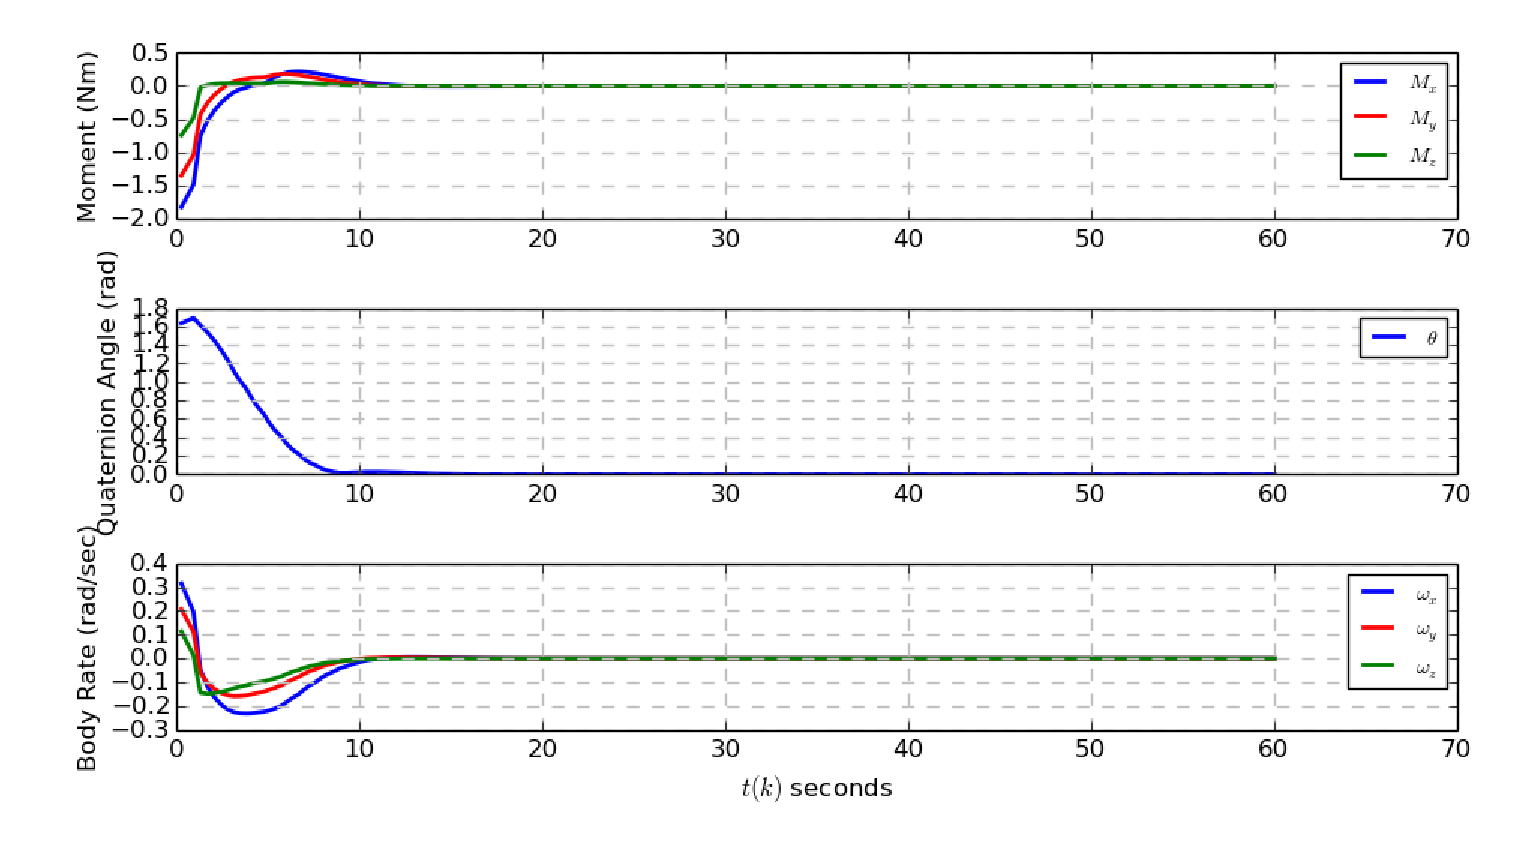
\psfig{file=figures/smc_attitude_and_rate_control.eps,width=6in}}
  \caption{SMC Attitude and Rate Control}
  \label{fig:SMCAttitudeAndRateControl}
\end{figure}
\begin{figure}[H]
  \centerline{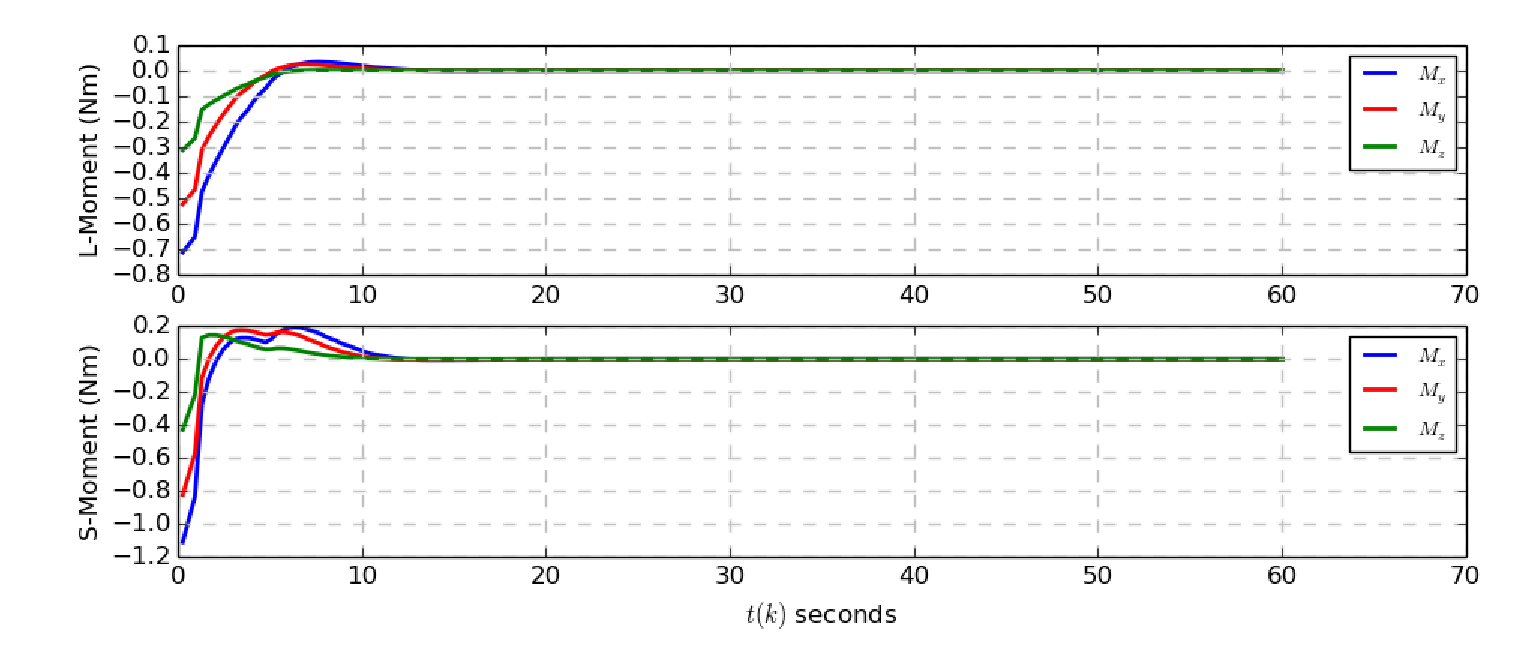
\psfig{file=figures/smc_attitude_and_rate_control_moments.eps,width=6in}}
  \caption{SMC Attitude and Rate Control Moments}
  \label{fig:SMCAttitudeAndRateControlMoments}
\end{figure}
As with the body rate comparative tests, the sliding mode controller shows a significant improvement in performance compared to the PID controller for the fixed attitude and body rate tests.  Section \ref{subsec:SpinStabilizedControl} follows up on these results by freeing up the motion about the $z$-axis for a spin-stabilized and nutation rejection test.

\subsection{Spin-Stabilized Control}
\label{subsec:SpinStabilizedControl}

This section verifies the ability for a controller to take the fixed attitude control problem from Section (\ref{subsec:FixedAttitudeControl}) and release the quaternion restriction on the rotational motion leaving the system to control five degrees of freedom $\omega_z = 0.314, \omega_x = \omega_y = 0$ and zero nutation about the $x$ and $y$ axes.  Since the Sliding Mode Controller has regularly out performed the PID controller, the spin-stabilized controller will run with control Equation (\ref{eqn:sliding_mode_control}) using the following parameters.
\begin{equation}
  \begin{aligned}
    L_q &= 0.01, \bs{L}_{\omega} = \bs{I} \begin{bmatrix} 0.398 & 0.383 & 0.416 \end{bmatrix}^T \\
    K_q &= 0.01, \bs{K}_{\omega} = \bs{I} \begin{bmatrix} 0.440 & 0.510 & 0.316 \end{bmatrix}^T \\
    S_q &= 0.01, S_{\omega} = 0.140
  \end{aligned}
\end{equation}

The initial convergence of to the spin stabilized state is rapid as in previous test configurations for the SMC.  In this case, the system remains with a steady state error.  Some manual gain tuning does not show any significant improvements and appears from the error measurements to be lagging behind the desired state and rocking back and forth about the desired spin axis.  Additional testing for gain tuning or improved visualizations such as the tPlot discussed in Section \ref{sec:ObjectOrientedNSSControlSystem} would help diagnose the source of the error.
\begin{figure}[H]
  \centerline{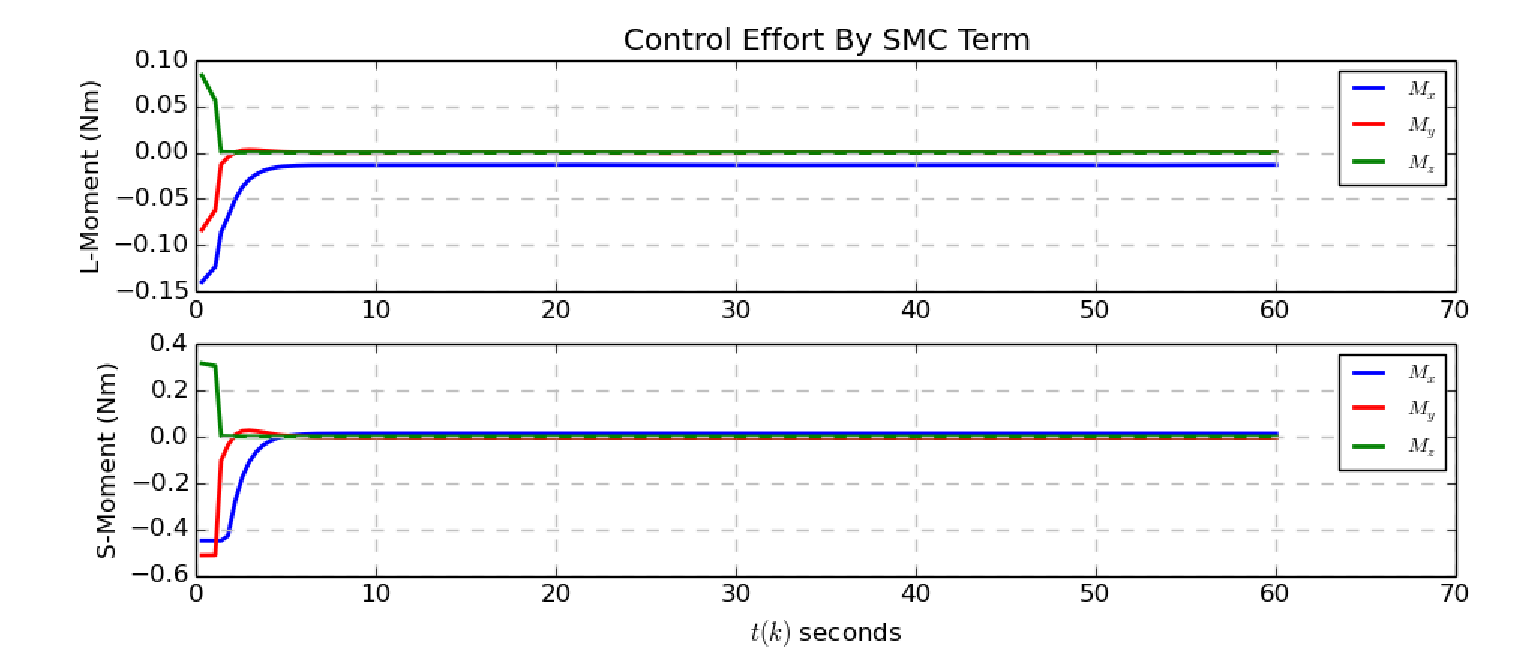
\psfig{file=figures/smc_nutation_and_rate_control.eps,width=6in}}
  \caption{SMC Nutation and Rate Control}
  \label{fig:SMCNutationAndRateControl}
\end{figure}
\begin{figure}[H]
  \centerline{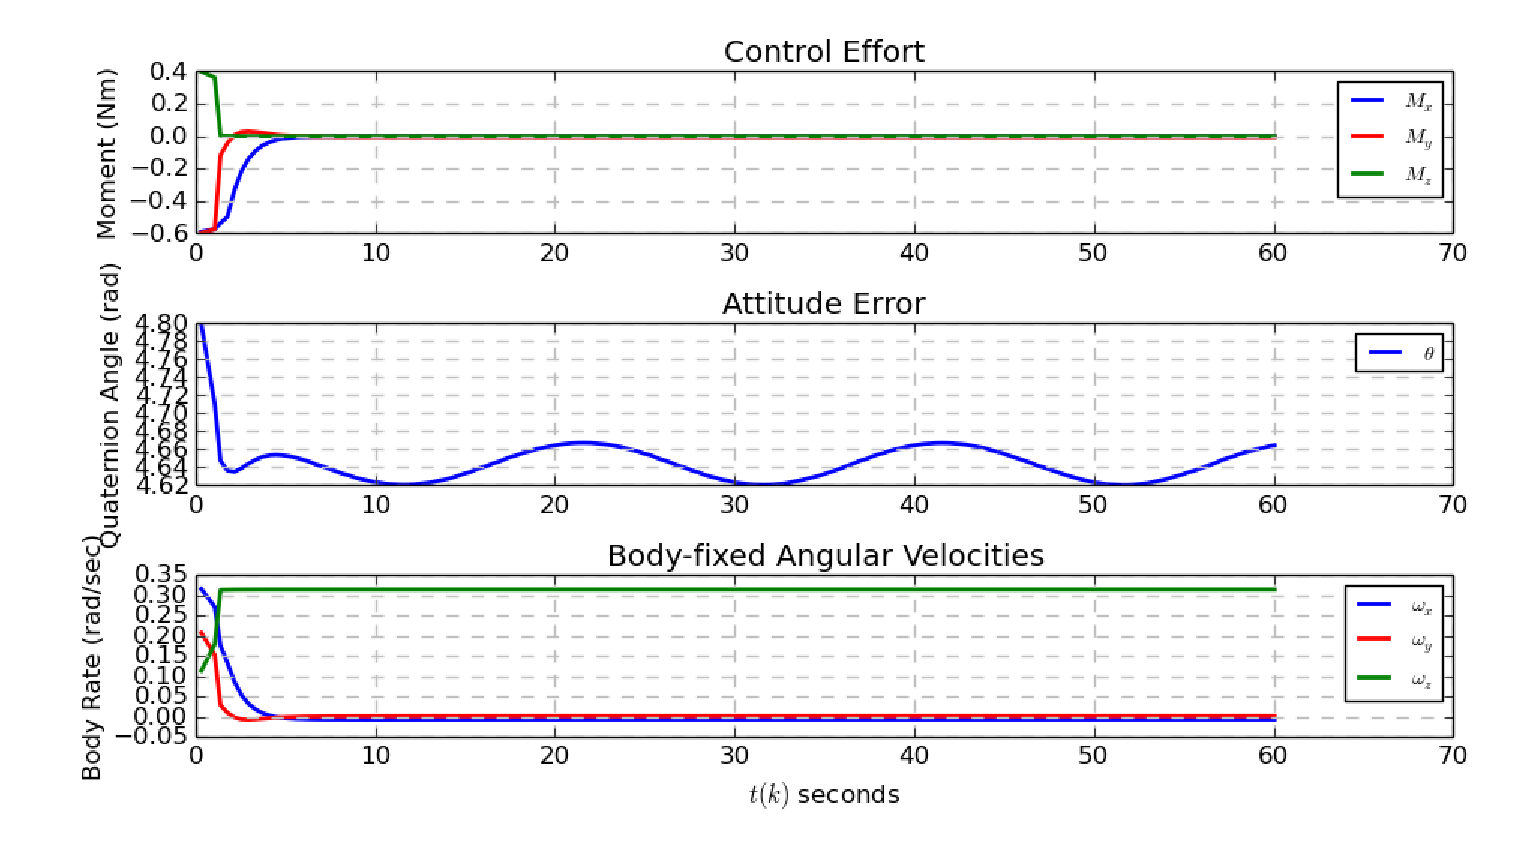
\psfig{file=figures/smc_nutation_and_rate_control_moments.eps,width=6in}}
  \caption{SMC Nutation and Rate Control Moments}
  \label{fig:SMCNutationAndRateControlMoments}
\end{figure}



\section{Messages Between TableSat and the Base Station}

\subsection{Message Protocol}
\label{subsec:UDPTCP}

Communication between the controller and the experimental TableSat is negotiated over a User Datagram Protocol (UDP) socket.  Both the controller and TableSat read and write over port 9877.  UDP is used for a stateless connection more generally used for pushing data over a large number of connections.  The other common communication protocol is Transmission Control Protocol (TCP) where a session is established between server and client and successful transferral of data is acknowledged by the recipient.

Advantages and disadvantages exist between the TCP and UDP protocols and became a critical factor in influencing the design of TableSat 1A base station controller. Section \ref{sec:NSSModel} goes into further detail in how this difference in protocols cropped up early in the development of the base station controller where the combination of a Numerical Simulation Software (like Matlab Simulink or Octave) with a UDP communication protocol produced a very fragile system.

A UDP message transmission is done in a ``fire and forget'' fashion.  The message header can generally include the originating hosts ip address and port so that the server knows where to send the response.  The session-less nature of UDP means that the originating server sends the message, but does not receive confirmation that the message transmitted successfully as with TCP where ever interaction is followed up with an acknowledgment from the other host.

The advantage to using UDP for the UNH TableSat 1 is that the satellite side code could be largely based off of Melissa Vess' work on her TableSat thesis where the control loop was implemented on-board, and the UDP connection was used to infrequently poll for data or modify sensor calibration values.  The UDP connection has the slight advantage of being able to transmit and receive packets without needing to wait for acknowledgments.  This could save a small fraction of time, but on modern hardware and with the small bandwidth usage this advantage is negligible.

Disadvantages to a UDP implementing the control interface through UDP include the possibility of packet loss where the sender submits a packet, but it gets corrupted or dropped.  Since UDP is a stateless connection, the sender doesn't wait for an acknowledgment which in this case would not come. This issue is handled by the communications module.  If the control loop rate on both updating the actuator voltages and polling sensor data is fast enough, a dropped packet would not matter much since a new updated set of values would be soon to follow.  Issues could be caused if the completion of a code loop was dependent on a packet coming in.  If dropped, the control loop could block until the next packet is received.  This was one issue encountered in the project version [sec:ControlLoopinSimulink].


\subsection{Message Definitions}
\label{subsec:MessageDefinitions}


The packet structure used for this project is the same as used by Melissa Vess \cite{vessthesis}. Each UDP packet is comprised of a packet header and data payload.  The packet header format remains constant for all messages containing five octets of data.

\begin{table}[H]
  \centering
  \begin{tabular}{| l | l |}
    \hline
    Header Octet & Description \\ \hline
    h1 & Message Number (0 to 255) \\ \hline
    h2 & Flags (0 - 255) \\ \hline
    h3 & Message Size (0 - 255) \\ \hline
    h4 & Message Size (0 - 255) \\ \hline
    h5 & 0 \\ \hline
  \end{tabular}
  \caption{UDP message headers}
  \label{tbl:UDPMessageHeaders}
\end{table}

The first octet (h1) contains the message number that matches to a predefined list of messages known by both the sender and recipient.  This is used to specify how the data in the payload is to be used.

The second octet (h2) is reserved for flags.  For some messages, flags can be set for additional data.  These are not used in the final implementation of NASA MMS TableSat 1A.

The third (h3) and fourth (h4) header octets define the size of the data's payload, so when reading data in from a buffer, the header can inform the recipient how many bytes need to get read in from the buffer in order to get to the end of the packet.  For payloads less than 256 bytes only the fourth header byte is needed.  For payloads larger than 255 bytes the following formula is used to specify the message size headers.

\begin{subequations}
  \begin{align}
    h4 &= mod(size, 256) \\
    h3 &= floor(size / 256)
  \end{align}
  \label{eqn:UDPSizeHeader}
\end{subequations}

The only meta data provided along with the payload beyond the data's size is an 8 bit message number.  Both UNH TableSat 1A and the control station have identical message list definitions.

\begin{table}[H]
  \centering
  \begin{tabular}{|l|l|l|l|}
    \hline
    Message Id & Payload Size & Data Type & Message Description \\ \hline
    2 & 1 octet & unsigned int & Set run mode \\ \hline
    4 & 1 octet & unsigned int & Set run mode \\ \hline
    18 & 4 x (8 octets) & float & Set fan voltages \\ \hline
    19 & 1 octet & unsigned int & Set log record mode \\ \hline
    20 & 1 octet & unsigned int & Request sensor reading \\ \hline
    22 & 1 octet & unsigned int & End of sensor log \\ \hline
    23 & 8 octets & float & Request sensor log data \\ \hline
    33 & 8 octets & float & Set log sample rate \\ \hline
    63 & 15 x (8 octets) & float & Sensor readings \\ \hline
    64 & 16 x (8 octets) & float & Sensor log entry \\ \hline
    65 & 8 octets & float & Sensor log size \\ \hline
    104 & 1 octet & unsigned int & Ack run mode \\ \hline
    118 & 1 octet & unsigned int & Ack fan volt \\ \hline
    119 & 1 octet & unsigned int & Ack sensor log run mode \\ \hline
    133 & 1 octet & unsigned int & Ack log sample rate \\ \hline
  \end{tabular}
  \caption{TableSat message definitions}
  \label{tbl:UDPMessageDefinitions}
\end{table}
